\documentclass[tikz,border=4pt]{standalone}

\usepackage{amsmath}
\usepackage{amssymb}
\usepackage{xcolor}
\usepackage{tikz}


\usetikzlibrary{
    arrows,
    arrows.meta,
    automata,
    backgrounds,
    calc,
    decorations.pathreplacing,
    fit,
    matrix,
    positioning,
    shapes,
    shapes.arrows,
    shapes.geometric,
    shapes.multipart
}



\tikzset{
  start/.style={
    rectangle,
    rounded corners,
    minimum width=3.5cm,
    minimum height=1cm,
    text centered,
    text width=3cm,
    draw=black,
    fill=green!20
  },
  stop/.style={
    rectangle,
    rounded corners,
    minimum width=3cm,
    minimum height=1cm,
    text centered,
    text width=2.5cm,
    draw=black,
    fill=red!20
  },
  decision/.style={
    diamond,
    aspect=2,
    minimum width=3cm,
    minimum height=1.2cm,
    text centered,
    text width=2.5cm,
    inner sep=1pt,
    draw=black,
    fill=yellow!20
  },
  process/.style={
    rectangle,
    minimum width=3cm,
    minimum height=1cm,
    text centered,
    text width=2.7cm,
    draw=black,
    fill=blue!10
  },
  arrow/.style={
    thick,
    -{Stealth}
  }
}


\usetikzlibrary{
  arrows.meta,
  positioning,
  shapes.geometric
}

\tikzset{
  start/.style={
    rectangle,
    rounded corners,
    minimum width=3.5cm,
    minimum height=1cm,
    text centered,
    text width=3cm,
    draw=black,
    fill=green!20
  },
  stop/.style={
    rectangle,
    rounded corners,
    minimum width=3cm,
    minimum height=1cm,
    text centered,
    text width=2.5cm,
    draw=black,
    fill=red!20
  },
  decision/.style={
    diamond,
    aspect=2,
    minimum width=3cm,
    minimum height=1.2cm,
    text centered,
    text width=2.5cm,
    inner sep=1pt,
    draw=black,
    fill=yellow!20
  },
  io/.style={
    trapezium,
    trapezium left angle=70,
    trapezium right angle=110,
    minimum width=3.5cm,
    minimum height=1cm,
    text centered,
    text width=3cm,
    draw=black,
    fill=blue!20
  },
  arrow/.style={
    thick,
    -{Stealth}
  }
}

\input{../jpk.inc}


\begin{document}

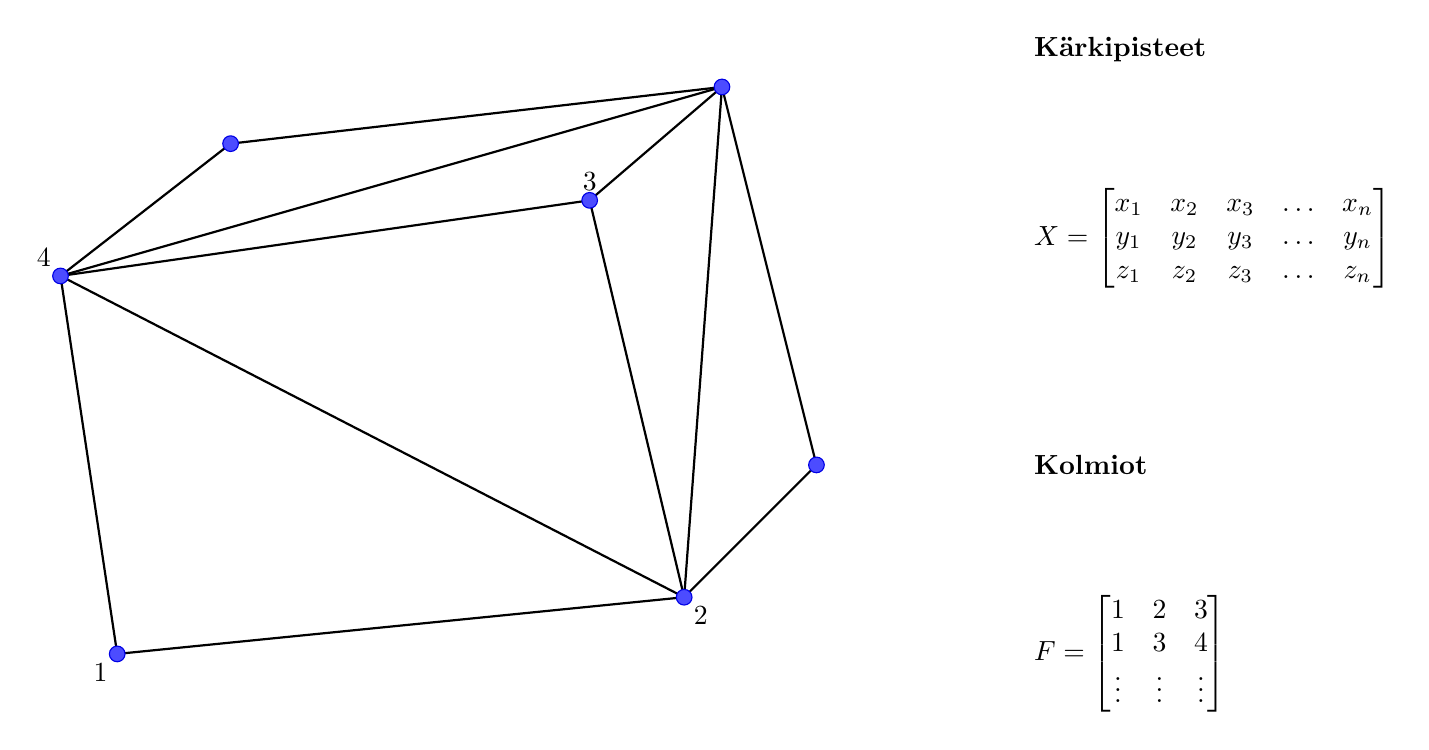
\begin{tikzpicture}[ 
  scale=2.4, 
  vertex/.style={ circle, fill=blue!70, draw=blue!90!black, inner sep=2pt }, 
  edge/.style={draw=black, thick}, 
  hidden/.style={draw=gray!60, dashed}, 
  label/.style={font=\small} ] 
\coordinate (P1) at (0,0); 
  \coordinate (P2) at (3,0.3); 
  \coordinate (P3) at (2.5,2.4); 
  \coordinate (P4) at (-0.3,2.0); 
  \coordinate (P5) at (0.9,0.8); 
  \coordinate (P6) at (3.7,1.0); 
  \coordinate (P7) at (3.2,3.0); 
  \coordinate (P8) at (0.6,2.7); 
\draw[edge] (P4)--(P2);
\draw[edge] (P1)--(P2)--(P3)--(P4)--cycle; 
\draw[edge] (P2)--(P6); 
  \draw[edge] (P3)--(P7); 
  \draw[edge] (P4)--(P8); 
  \draw[edge] (P6)--(P7); 
  \draw[edge] (P7)--(P8); 
\draw[edge] (P2)--(P7); 
  \draw[edge] (P4)--(P7); 
\node[vertex] at (P1) {}; 
  \node[below left] at (P1) {$1$}; 
  \node[vertex] at (P2) {}; 
  \node[below right] at (P2) {$2$}; 
  \node[vertex] at (P3) {}; 
  \node[above] at (P3) {$3$}; 
  \node[vertex] at (P4) {}; 
  \node[above left] at (P4) {$4$}; 
\node[vertex] at (P6) {}; 
\node[vertex] at (P7) {}; 
\node[vertex] at (P8) {}; 
\node[anchor=west, align=left] at (4.8,3.2) { \textbf{Kärkipisteet} }; 
  \node[anchor=west] at (4.8,2.2) { 
    $ \V{X} = \begin{bmatrix} 
      x_1 & x_2 & x_3 & \dots & x_n\\
      y_1 & y_2 & y_3 & \dots & y_n\\
      z_1 & z_2 & z_3 & \dots & z_n\\
    \end{bmatrix} $ }; 
\node[anchor=west, align=left] at (4.8,1.0) { \textbf{Kolmiot} };
  \node[anchor=west] at (4.8,0.0) { $ \V{F} = \begin{bmatrix} 1 & 2 & 3\\ 1 & 3 & 4\\ \vdots & \vdots & \vdots \end{bmatrix} $ }; 
\end{tikzpicture}

\end{document}
